\documentclass[tikz, border=3mm, convert={outfile=r-decomposed.png}]{standalone}

\usetikzlibrary{
  matrix,
  positioning
}

\begin{document}

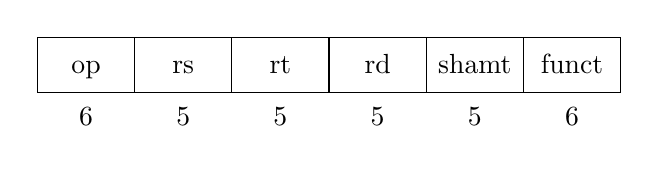
\begin{tikzpicture}[node distance=1em]

\matrix (decomposed-representation) [
  matrix of nodes,
  row sep=0.2em,
  column sep=-\pgflinewidth,
  row 1/.style={
    nodes={
      rectangle, 
      draw, 
      text centered,
          text width=10mm,
      anchor=base,
      text height=.8em,text depth=.2em,minimum size=7mm
    }
  }
] {
op & rs & rt & rd & shamt & funct \\
6 & 5 & 5 & 5 & 5 & 6 \\
};

\end{tikzpicture}

\end{document}
